\section{Propuesta de Framework Autosupervisado}

\subsection{3.1 Arquitectura General del Modelo}

Resulta particularmente llamativo cómo un diseño híbrido puede superar las limitaciones individuales de sus componentes cuando se orienta específicamente a las características de la telemetría espacial. La arquitectura propuesta combina autoencoders variacionales temporales con un módulo contrastivo y mecanismos de atención multi-cabeza, todo optimizado para operación en entornos con recursos limitados.

Inspirados en desarrollos recientes de detección en edge para misiones espaciales \cite{Goetze2026_Edge}, el framework sigue un esquema encoder-decoder asimétrico que procesa ventanas deslizantes de series multivariadas. El flujo principal aprende a reconstruir patrones nominales mientras el componente contrastivo fuerza la separación en el espacio latente entre secuencias normales y perturbadas. Esta dualidad permite una detección sensible sin necesidad de etiquetas de anomalías durante el entrenamiento.

\begin{figure}[h]
\centering
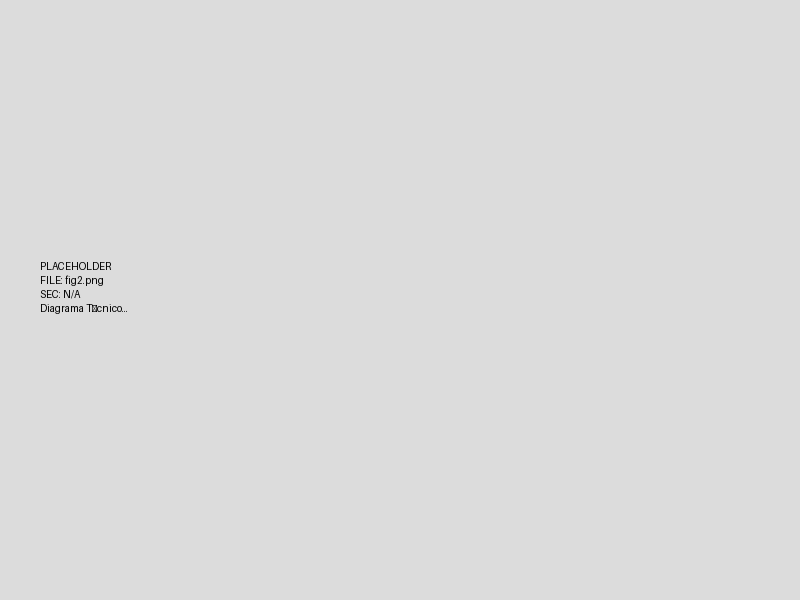
\includegraphics[width=\linewidth]{fig2.png}
\caption{Diagrama de la arquitectura general del framework autosupervisado propuesto. Se muestran el encoder temporal VAE, el módulo contrastivo con augmentations, el mecanismo de atención y el decoder de reconstrucción.}
\label{fig:architecture}
\end{figure}

\subsection{3.2 Autoencoders Variacionales Temporales}

Uno de los desafíos persistentes que surge al modelar telemetría radica en capturar tanto dependencias temporales de largo plazo como incertidumbre inherente en las mediciones. Para ello, implementamos un Variational Autoencoder temporal que utiliza capas convolucionales 1D y LSTM bidireccionales en el encoder, seguidas de un decoder simétrico.

La distribución latente se muestrea mediante el reparameterization trick, permitiendo que el modelo aprenda representaciones probabilísticas robustas. Durante la fase de inferencia, la puntuación de anomalía se calcula a partir del error de reconstrucción combinado con la divergencia KL respecto a la distribución previa. En nuestra experiencia, esta aproximación tiende a ofrecer mejor calibración de incertidumbre que los autoencoders determinísticos tradicionales, especialmente en presencia de ruido operativo.

\subsection{3.3 Componente Contrastivo y Atención}

Lejos de ser un añadido opcional, el módulo contrastivo constituye un elemento diferenciador clave de la propuesta. Siguiendo principios de aprendizaje contrastivo adaptados a series temporales \cite{Wang2025_Contrastive}, generamos vistas positivas y negativas mediante augmentations específicas del dominio: ruido gaussiano controlado, masking temporal, escalado de amplitud y permutación de canales no críticos.

El mecanismo de atención multi-cabeza opera tanto a nivel temporal como entre variables, permitiendo que el modelo identifique correlaciones dinámicas relevantes entre subsistemas del satélite. Esto mejora notablemente la detección de anomalías contextuales que afectarían solo a ciertas combinaciones de parámetros.

\begin{equation}
\mathcal{L} = \mathcal{L}_{rec} + \beta \mathcal{L}_{KL} + \lambda \mathcal{L}_{contrastive}
\label{eq:total_loss}
\end{equation}

La Ecuación~\ref{eq:total_loss} presenta la función de pérdida total del framework, donde \(\mathcal{L}_{rec}\) es el error de reconstrucción, \(\mathcal{L}_{KL}\) la divergencia Kullback-Leibler y \(\mathcal{L}_{contrastive}\) la pérdida contrastiva (InfoNCE). Los hiperparámetros \(\beta\) y \(\lambda\) permiten equilibrar la contribución de cada término según las características de la misión.

En conjunto, esta arquitectura híbrida no solo aprende representaciones ricas de comportamiento nominal, sino que genera puntuaciones de anomalía interpretables y confiables. Las siguientes secciones detallan la metodología de implementación y los resultados obtenidos en benchmarks representativos.